\documentclass[pstricks,border=11pt]{article}

\hfuzz=0.64pt
\usepackage[utf8]{inputenc}

\usepackage{amsmath} % for the equation* environment
\usepackage{tabularx}
\usepackage{multirow} % Required for multirows
\usepackage{booktabs} % For prettier tables
\usepackage{siunitx} % Required for alignment
\usepackage{pgfplots}
\usepackage{pst-plot}
\usepackage{hyperref}
\pgfplotsset{compat = newest}
\sisetup{
  round-mode          = places, % Rounds numbers
  round-precision     = 2, % to 2 places
}
\title{Polynomial Functions Menu Task}
\author{Tiffany Pham}
\date{18 February 2023}

\begin{document}

\maketitle

\section{Introduction}
Build as \textit{few} polynomial functions as possible to satisfy each constraint at least once.
\vspace{5mm}
\begin{center}
Record your functions in factored form or expanded form.
\end{center}

\begin{table}[!ht]
\begin{tabular}{|l|p{2in}|l|p{2in}|} 
\hline
A. & Has 2 negative x-intercepts                                & B. & Never enters Quadrant I                \\ 
\hline
C. & Has a positive y-intercept & D. & Ends in Quadrant I         \\ 
\hline
E. & Opens down                & F. & Three x-intercepts           \\ 
\hline
G. & Has an x-intercept with a multiplicity of 2                     & H. & Is symmetrical  \\
\hline
\end{tabular}
\end{table}
\begin{center}
    \textit{Which constraints pair nicely?}
    
    \textit{Which constraints cannot be paired?}
    
    \textit{Is it possible to solve in 2, 3, or 4 polynomial functions?}
\end{center}

A, C, D, F, G, and H pair nicely, and B, and E pair nicely. The ones you can't pair are B and D because the function will have to end in Quadrant I to fulfill the requirement of D, but it can never enter Quadrant I in order to fulfill the requirement of B, so these two will never be able to work together. 

I built two functions that fit all of the constraints. One function for A, C, D, F, G, and H, and another for B and E. Since I've built two functions, I think the least functions that this problem can have is two because both of my functions have satisfied all of the constraints.

\vspace{15mm}
\section{Functions}
Describe how and why you built each function. Be sure to identify which polynomial functions satisfy which constraints.

\hfill \break
Function 1
\hfill \break
Satisfies: A, C, D, F, G, H
\begin{displaymath}
    y=-((2x)^2-(x)^4-2)   
\end{displaymath}

\vspace{5mm}
\begin{center}
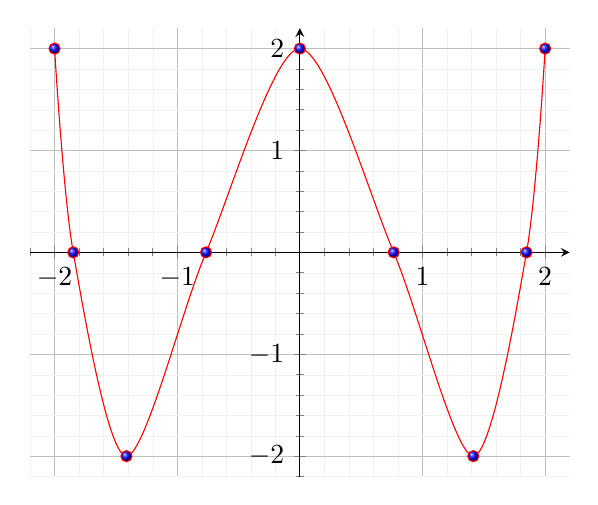
\begin{tikzpicture}
  \begin{axis}%
    [grid=both,
     minor tick num=4,
     grid style={line width=.1pt, draw=gray!10},
     major grid style={line width=.2pt,draw=gray!50},
     axis lines=middle,
     enlargelimits={abs=0.2}
    ]
    \addplot [domain=-2:2,samples=100,smooth,red,mark=ball]
    % dashed option draws the dashed curve. You can also use dotted, dashdotted, dashdotdotted.  
      coordinates { (-2,2) (-1.8478,0) (-1.414,-2) (-0.765,0) (0,2) (0.765,0) (1.414,-2) (1.848,0) (2,2) };   
  \end{axis}
\end{tikzpicture}
\end{center}
\vspace{5mm}

For this polynomial function, I made it have at least 2 negative x-intercepts (-1.8478,0) and (-0.765,0) which fulfilled requirement A. It also has a positive y-intercept (0,2) which fulfilled requirement C. It also ends in quadrant I/ goes on forever in quadrant I, which fulfilled requirement D, and alongside the two negative x-intercepts, it also had two more positive x-intercepts. The x-intercepts are the same, but they are the opposite on the other side: (0.765,0) and (1.848,0). This fulfilled requirement F of having at least three x-intercepts. Since the x-intercepts were the opposite of each other but were on the same point, it meant that this polynomial function was symmetrical which fulfilled the requirement of H. Lastly, to fulfill G I made it have a multiplicity of two by adding the exponent of 2 to $(2x)$.


\vspace{35mm} %5mm vertical space
\hfill \break
Function 2
\hfill \break
Satisfies: B, E
\begin{displaymath}
    y=-(x+2)(x+2)
\end{displaymath}

\vspace{5mm}
\begin{center}
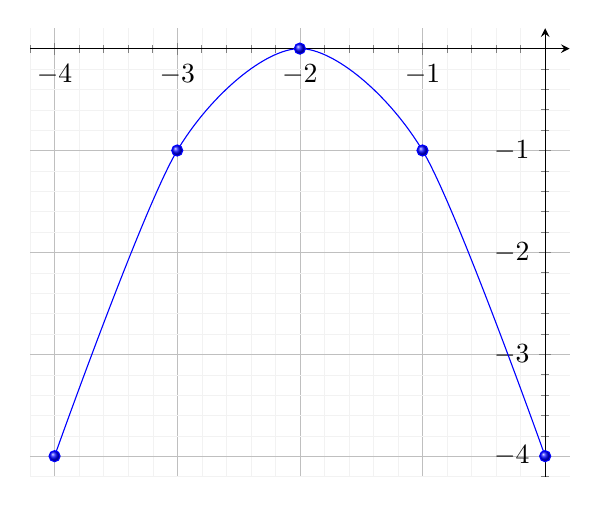
\begin{tikzpicture}
  \begin{axis}%
    [grid=both,
     minor tick num=4,
     grid style={line width=.1pt, draw=gray!10},
     major grid style={line width=.2pt,draw=gray!50},
     axis lines=middle,
     enlargelimits={abs=0.2}
    ]
    \addplot [domain=-4:0,samples=100,smooth,blue,mark=ball]
    % dashed option draws the dashed curve. You can also use dotted, dashdotted, dashdotdotted.  
      coordinates { (-4,-4) (-3,-1) (-2,0) (-1,-1) (0,-4) };   
  \end{axis}
\end{tikzpicture}
\end{center}
\vspace{5mm}

For this other polynomial function, I made sure that it never entered quadrant I, which is the top right corner and I added the negative to the \textit{A} variable which made it open down which fulfilled both requirements of B and E.

\vfill
\hfill \break
\textbf{Desmos Graphs for better reference}
\hfill \break
\url{https://www.desmos.com/calculator/4dichxj22j}

\end{document}
